\documentclass[11pt,letterpaper]{article}
\usepackage[lmargin=1in,rmargin=1in,bmargin=1in,tmargin=1in]{geometry}
\usepackage{style/quiz}
\usepackage{style/commands}

% -------------------
% Content
% -------------------
\begin{document}
\thispagestyle{title}

% Quiz 1
\quizsol \textit{True/False}: The number 1 is prime. \pspace

\sol The statement is \textit{false}. A prime number is an integer greater than 1 that can only be factored as the product of one and itself. So for example, the integer 11 is prime because we can only factor 11 as $11= 1 \cdot 11$. However, the integer 12 is not prime because we can write $12= 2 \cdot 6$, neither of which are 1 or 12. \pvspace{1.5cm}



% Quiz 2
\quizsol \textit{True/False}: $\gcd(2^3 \cdot 3 \cdot 5, 2 \cdot 3^2 \cdot 7)= 2^3 \cdot 3^2 \cdot 5 \cdot 7$. \pspace

\sol The statement is \textit{false}. Remember given a prime factorization of the numbers, we find the gcd by choosing the \textit{smallest} powers of each prime that appears in the factorizations. So we should have $\gcd(2^3 \cdot 3 \cdot 5, 2 \cdot 3^2 \cdot 7)= 2 \cdot 3$. Instead, the largest power of each prime that appears in the factorizations was chosen which is how we compute the lcm. Therefore, we have $\lcm(2^3 \cdot 3 \cdot 5, 2 \cdot 3^2 \cdot 7)= 2^3 \cdot 3^2 \cdot 5 \cdot 7$. \pvspace{1.5cm}



% Quiz 3
\quizsol \textit{True/False}: $\sqrt[3]{2^8 \cdot 3^3 \cdot 5^1 \cdot 7^5}= 2^2 \cdot 3^1 \cdot 7 \sqrt[3]{2^2 \cdot 5^1 \cdot 7^2}$ \pspace

\sol The statement is \textit{true}. There are two ways to think about this. First, we should write out the numbers and group them into threes and pull out/leave the terms appropriately:
	\[
	\sqrt[3]{2^8 \cdot 3^3 \cdot 5^1 \cdot 7^5}= \sqrt[3]{\underline{2 \cdot 2 \cdot 2} \cdot \underline{2 \cdot 2 \cdot 2} \cdot 2 \cdot 2 \cdot \underline{3 \cdot 3 \cdot 3} \cdot 5 \cdot \underline{7 \cdot 7 \cdot 7} \cdot 7 \cdot 7}= 2^2 \cdot 3^1 \cdot 7 \sqrt[3]{2^2 \cdot 5 \cdot 7^2}
	\]
Alternatively, we can use division. We know that $8/3$ is 2 with remainder 2, $3/3$ is 1 with remainder 0, $1/3$ is 0 with remainder 1, and $5/3$ is 1 with remainder 2. So we can pull out two 3's with 2 remaining, one 3 with 0 remaining, no 5's with 1 remaining, and two 7's with 2 remaining, which gives:
	\[
	\sqrt[3]{2^8 \cdot 3^3 \cdot 5^1 \cdot 7^5}= 2^2 \cdot 3^1 \cdot 7 \sqrt[3]{2^2 \cdot 5^1 \cdot 7^2}
	\] \pvspace{1.5cm}



% Quiz 4 
\quizsol \textit{True/False}: 68 increased by 119\% is $68(1.19)$. \pspace

\sol The statement is \textit{false}. To find 119\% of 68, we would multiply 68 by the percent written as a decimal. This would be $68(1.19)$. However, to increase or decrease a number by a percentage, we compute the number $\#(1 \pm \%)$, where we add if we are increasing, subtract if we are decreasing, $\#$ is the number, and \% is the percentage written as a decimal. So to increase 68 by 119\%, we need to compute $68(1 + 1.19)= 68(2.19)$. \pvspace{1.5cm}



\newpage



% Quiz 5
\quizsol \textit{True/False}: If $f(x)= 3x + 5$ and $g(x)= 1 - 2x$, then $(f \circ g)(1)= 8$. \pspace

\sol The statement is \textit{false}. Recall that $(f \circ g)(1)= f(g(1))$. First, we compute $g(1)$: $g(1)= 1 - 2(1)= 1 - 2= -1$. Then we need to compute $f(g(1))= f(-1)$. We have $f(-1)= 3(-1) + 5= -3 + 5= 2$. \pvspace{1.5cm}



% Quiz 6
\quizsol \textit{True/False}: The point $(1, -3)$ is on the graph of $f(x)= x - 3$. \pspace

\sol The statement is \textit{false}. We have the point $(x, y)= (1, -3)$. If this point is on the graph of $f(x)$, then these $x$ and $y$ satisfy the equation for $f(x)$. We can check this:
	\[
	\begin{aligned}
	f(x)&= x - 3 \\
	-3&= 1 - 3 \\
	-3&\neq -2
	\end{aligned}
	\]
Therefore, the point $(1, -3)$ is not on the graph of $f(x)$. Alternatively, if $x= 1$, then the corresponding point on the graph of $f(x)$ would have $y$-value $f(1)= 1 - 3= -2$. Then the point $(1, -2)$ is on the graph of $f(x)$. But then $(1, -3)$ is not on the graph of $f(x)$. \pvspace{1.5cm}



% Quiz 7
\quizsol \textit{True/False}: The graph of the solutions to $2x - 6y= 9$. \pspace

\sol The statement is \textit{true}. The graph of the set of solutions to an equation of the form $Ax + By= C$ is a line. Here we have $A= 2$, $B= -6$, and $C= 9$. Notice also we can solve for $y$:
	\[
	\begin{aligned}
	2x - 6y&= 9 \\
	-6y&= -2x + 9 \\
	y&= \frac{-2}{-6}\,x + \frac{9}{-6} \\
	y&= \frac{1}{3}\,x - \frac{3}{2}
	\end{aligned}
	\]
The function $f(x)= \frac{1}{3}x - \frac{3}{2}$ is a linear function, whose graph must be a line. \pvspace{1.3cm}



% Quiz 8
\quizsol \textit{True/False}: The line through $(-1, 5)$ with slope 3 is $y= 3x + 8$. \pspace

\sol The statement is \textit{true}. We know that the line contains the $(-1, 5)$ and has slope 3, i.e. $m= 3$. Then we have
	\[
	\begin{aligned}
	y&= mx + b \\
	y&= 3x + b \\
	5&= 3(-1) + b \\
	5&= -3 + b \\
	b&= 8 
	\end{aligned}
	\]
Therefore, the equation of the line is $y= 3x + 8$. 



\newpage



% Quiz  9
\quizsol \textit{True/False}: A function cannot have two $y$-intercepts. \pspace

\sol The statement is \textit{true}. If a function had two $y$-intercepts, then there would be two points on the graph of the function on the $y$-axis. But then the function would fail the vertical line test---which is impossible because it is a function. \pvspace{1.3cm}



% Quiz  10
\quizsol \textit{True/False}: $47$ increased by $16\%$ is $47(0.16)$. \pspace

\sol The statement is \textit{false}. There are two ways to do this: first, we can use the percent increase/decrease formula; that is, if we want to increase/decrease a number by a percentage, we use the formula $\#(1 \pm \%)$, where $\#$ is the number, $\%$ is the percentage written as a decimal, and we choose $+$ if we are increasing the number and $-$ if we are decreasing the number. So in our case, we have $47(1 + 0.16)= 47(1.16)$. The other method is to find the amount of increase/decrease and then add/subtract this to our original number, respectively. We want to find $16\%$ of $47$, which is $47(0.16)$. Then we increase, i.e. add, this to our original number, so we have $47 + 47(0.16)= 47(1 + 0.16)= 47(1.16)$. \pvspace{1.3cm}



% Quiz 11
\quizsol \textit{True/False}: The vertex of the quadratic function $y= (x + 2)^2 - 3$ is the point $(2, -3)$. \pspace

\sol The statement is \textit{false}. The $x$-coordinate of the vertex is the $x$-value that makes the square term zero. In this case, $x= -2$ would make $(x + 2)^2$ zero. Then we would be left with $y= -3$, which is the $y$-coordinate of the vertex. Therefore, the vertex is $(-2, -3)$. Alternatively, the `proper' vertex form of a quadratic function is $y= A(x - B) + C$. The vertex is $(B, C)$. Writing the `proper' vertex form of the quadratic function $y= (x + 2)^2 - 3$, we have $y= (x - \;-2)^2 + (-3)$. Therefore, the vertex form is $(-2, -3)$. Finally, one could expand this out: $y= (x + 2)^2 - 3= (x^2 + 4x + 4) - 3= x^2 + 4x + 1$. The $x$-coordinate of the vertex is $x= \frac{-b}{2a}= \frac{-4}{2(1)}= -2$. Then the $y$-coordinate of the vertex is $y(-2)= (-2)^2 + 4(-2) + 1= 4 - 8 + 1= -3$. Therefore, the vertex is $(-2, -3)$. \pvspace{1.3cm}



% Quiz 12
\quizsol \textit{True/False}: $x^2 - 4x - 5= (x + 1)(x - 5)$ \pspace

\sol The statement is \textit{true}. One way of seeing this would be to expand $(x + 1)(x - 5)$,
	\[
	(x + 1)(x - 5)= x^2 - 5x + x - 5= x^2 - 4x - 5.
	\]
Alternatively, we can factor the polynomial $x^2 - 4x - 5$. First, we find the factors of $5$, which are only $1, 5$. Because the 5 is negative, the factors must have opposite signs. 
	\[
	\begin{aligned}
	1, -5&\colon -4 \\
	-1, 5&\colon \phantom{-..}4
	\end{aligned}
	\]
We want these signed factors to add to $-4$. Therefore, we want `factors' $1, -5$. Therefore, 
	\[
	x^2 - 4x - 5= (x + 1)(x - 5)
	\]



\newpage



% Quiz 13
\quizsol \textit{True/False}: $2x^2 + 11x - 6= (2x - 1)(x + 6)$ \pspace

\sol The statement is \textit{true}. There are two approaches: first, we can simply expand the right side and show that this is equal to the left side, 
	\[
	(2x - 1)(x + 6)= 2x^2 + 12x - x - 6= 2x^2 + 11x - 6
	\]
Alternatively, we can factor the polynomial on the left side and show that it is the same as the given factorization of the right side, \pspace
	\[
	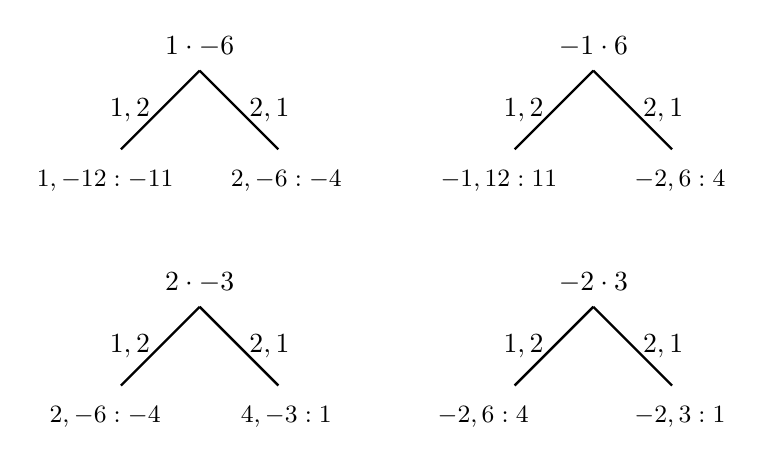
\begin{tikzpicture}
	\node at (0,0) {$1 \cdot -6$};
	\draw[line width=0.03cm] (0,-0.3) -- node[left] {$1, 2$} ++ (-1,-1);
	\draw[line width=0.03cm] (0,-0.3) -- node[right] {$2, 1$} ++ (1,-1);
	\node at (-1.2,-1.7) {\small$1, -12: -11$};
	\node at (1.1,-1.7) {\small$2, -6: -4$};
	
	\node at (5,0) {$\boxed{-1 \cdot 6}$};
	\draw[line width=0.03cm] (5,-0.3) -- node[left] {$1, 2$} ++ (-1,-1);
	\draw[line width=0.03cm] (5,-0.3) -- node[right] {$2, 1$} ++ (1,-1);
	\node at (3.8,-1.7) {\small$\boxed{-1, 12: 11}$};
	\node at (6.1,-1.7) {\small$-2, 6: 4$};
	
	\node at (0,-3) {$2 \cdot -3$};
	\draw[line width=0.03cm] (0,-3.3) -- node[left] {$1, 2$} ++ (-1,-1);
	\draw[line width=0.03cm] (0,-3.3) -- node[right] {$2, 1$} ++ (1,-1);
	\node at (-1.2,-4.7) {\small$2, -6: -4$};
	\node at (1.1,-4.7) {\small$4, -3: 1$};
	
	\node at (5,-3) {$-2 \cdot 3$};
	\draw[line width=0.03cm] (5,-3.3) -- node[left] {$1, 2$} ++ (-1,-1);
	\draw[line width=0.03cm] (5,-3.3) -- node[right] {$2, 1$} ++ (1,-1);
	\node at (3.6,-4.7) {\small$-2, 6: 4$};
	\node at (6.1,-4.7) {\small$-2, 3: 1$};
	\end{tikzpicture}
	\]	
Therefore,
	\[
	2x^2 + 11x - 6= (2x - 1)(x + 6)
	\] \pvspace{1.3cm}


% 14: the vertical asympotes of f= (x-1)(x+3) / (x-1)(x+5) are x= 1 and x=-5
% 15 To add $\dfrac{5}{x + 1}$ and $\dfrac{x}{(x + 1)^2}$, one would use the common denominator of $x + 1$.
% 16: there is no function with domain all reals and a vertical asymptote at $x= 1$. 









\end{document}